% !TeX root = ../../../main.tex
\begin{figure}[htbp]
\begin{ChSixFloatBody}

\scriptsize
    \centering
    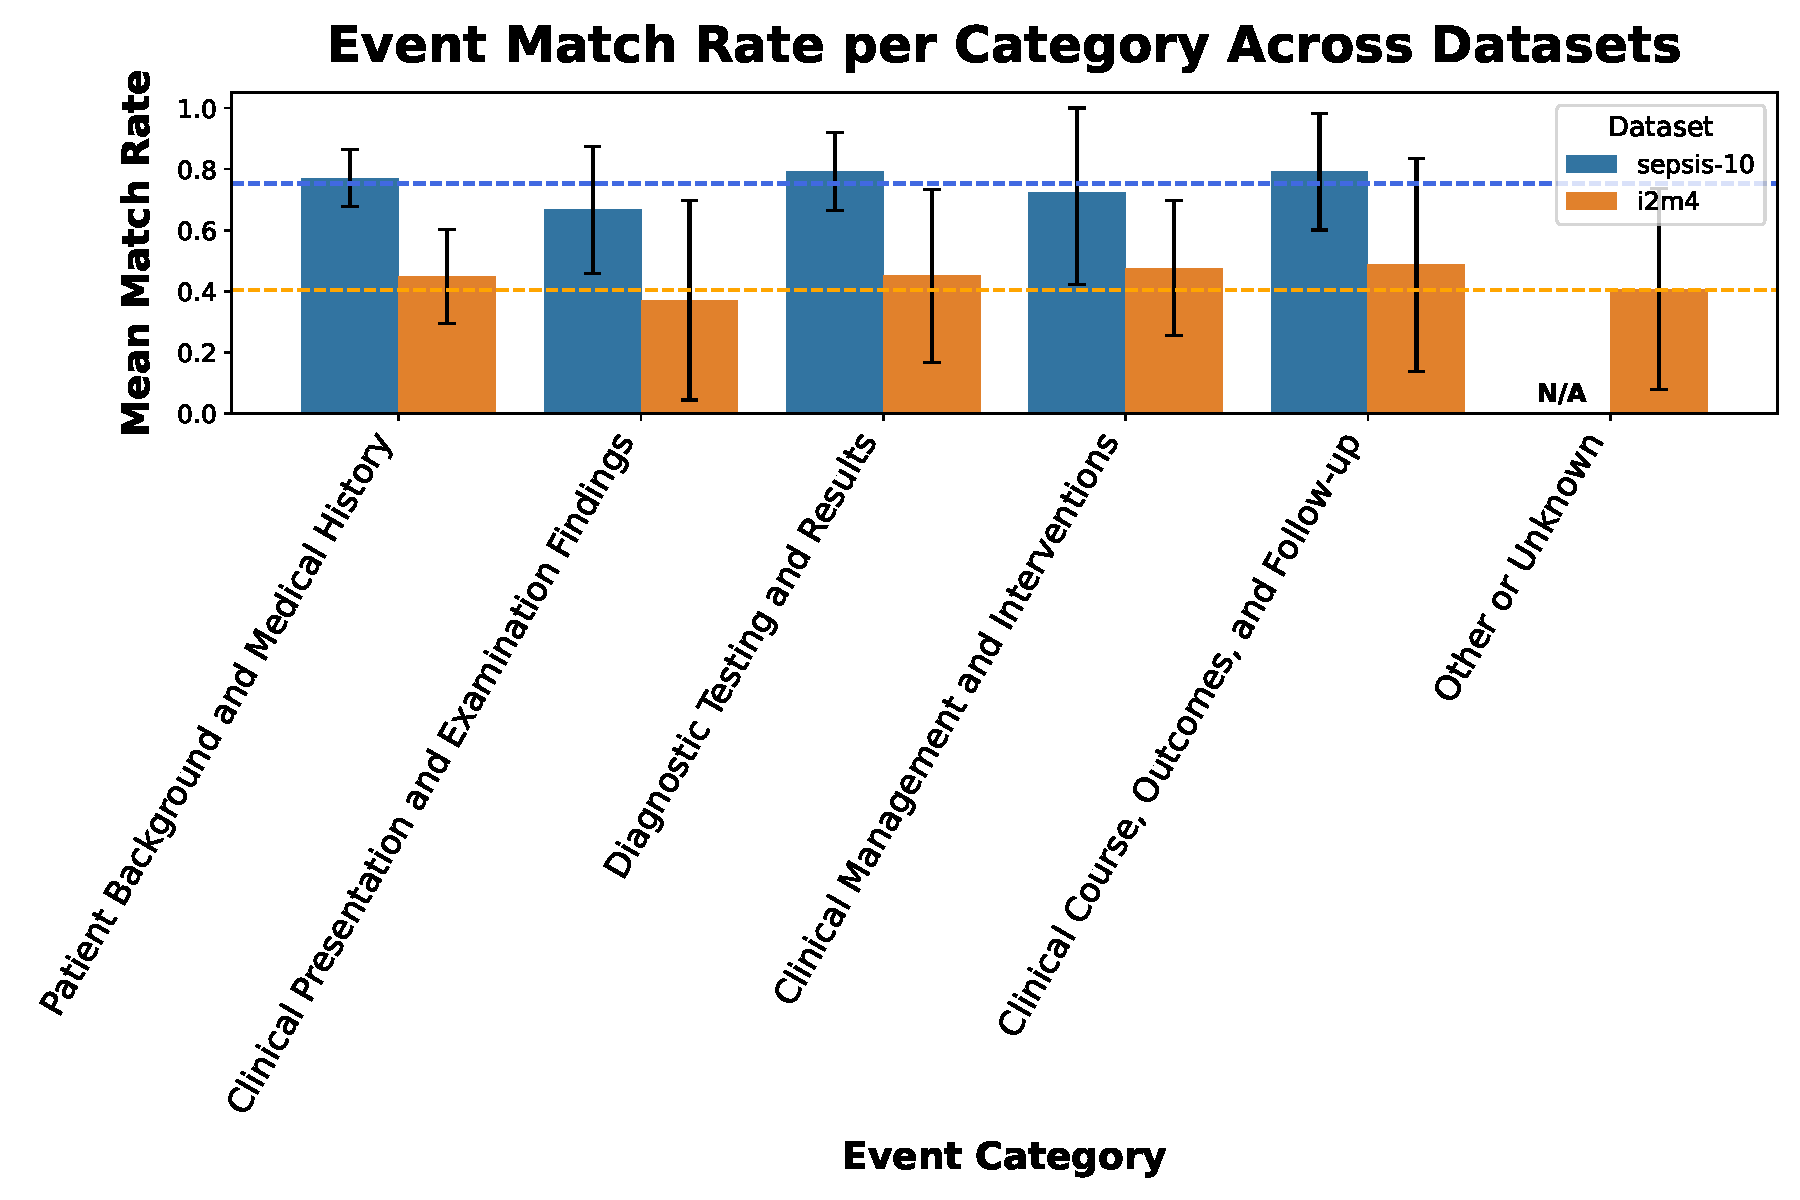
\includegraphics[width=0.9\linewidth]{Appendices/appendix-ch06/images/figures/event_match_rate_per_category.pdf}
    
    

\end{ChSixFloatBody}
\caption{Mean event match rate across predefined event type categories for the i2m4 and \texttt{sepsis-10} datasets.  
    Bars represent the mean match rate for each event type category, calculated as the proportion of aligned event pairs (between the manual annotator and Llama 3.3) with cosine distance less than the matching threshold.  
    Error bars indicate the standard deviation of match rates across case reports.  
    The dashed lines represent the overall mean match rates for each dataset across all categories (From Table~\ref{ch06:tab:results}: \textcolor{blue}{\texttt{sepsis-10}}: 0.753 and \textcolor{orange}{i2m4}: 0.404)
    The ``Other or Unknown'' category is absent in \texttt{sepsis-10}, resulting in no match rate for this category in that dataset.}\ChSixFloatLabel{ch06:fig:event_match_rate_per_category}
\end{figure}